\section{Planeamiento militar} \todo{Mejor tratar del PICB}
... El título es genérico

\section{Preparación de Inteligencia del Campo de Batalla (PICB)}
El diseño, análisis y ejecución de las operaciones militares consta de cinco fases:
\begin{enumerate}
\item Recepción de la misión.
\item Análisis de la misión.
\item Desarrollo del conocimiento de la operación.
\item Desarrollo de los planes y órdenes.
\item Supervisión y control.
\end{enumerate}

Durante el desarrollo de las fases se realizan un conjunto de actividades que tienen como objetivo documentar y analizar el \gls{campo} de batalla. Así, la \emph{recepción de la misión} comprende las actividades:\todo{Refinar toda la lista.}
\begin{enumerate}
\item Reorganización de las secciones del \gls{estado-mayor}.
\item Reunión del \gls{estado-mayor} (lugar, fecha, hora).
\item Reunir las herramientas.
\item Actualización de la información disponible.
\item Realizar evaluación inicial.
\item Guía inicial del Comandante (Diseño).
\item Formulación de la orden preparatoria.
\end{enumerate}

Para la presente tesis, es el \emph{análisis de la misión} la fase en la que se trabajará. Donde se desarrolla la \gls{picb} \todo{Mejorar texto.}

\begin{enumerate}
\item Intención.
\item Estado final deseado.
\item Criterios de finalización.
\item Condiciones de éxito.
\item Objetivos.
\item Hipótesis.
\end{enumerate}

Las fases del \gls{picb} son: \todo{Creo que mejor quitar el detalle de lista.}

\begin{enumerate}
\item Determinación, evaluación y análisis del campo de batalla.
  \begin{itemize}
  \item Zona de Acción o Sector Defensivo,
  \item Área de Influencia y
  \item Área de Interés.
  \end{itemize}

\item Análisis del terreno  y de las  condiciones meteorológicas.

\item Análisis del enemigo.
  \begin{itemize}
  \item Dispositivo,
  \item Composición,
  \item Fuerza,
  \item Actividades reveladoras recientes y actuales,
  \item Peculiaridades y deficiencias.
  \end{itemize}

\item Integración (Establecer capacidad del enemigo, calco de eventos y calco de apoyo a la decisión).
\end{enumerate}


%% >>>

\section{Operaciones militares}
\todo{¿Mejor como otra sección?}
\todo{Agregar la fuente (el experto) como prosa.}
\todo{Creo que mejor va antes de la PICB.}

La operaciónes militares aplican principios acerca de la conducción de la unidades en el campo de combate. Dichas unidades pueden ser tropas de infantería, tanques, aviones, entre otros. Para realizar la conducción de la operación, las unidades ejecutan una serie de actividades definidas por la \gls{operacion}. El empleo efectivo de las unidades puede ser efectuado mediante el uso de principios, que sirven de guía al momento de realizar el análisis del \gls{escenario} de batalla. Estos principios se basan en la descripción que se tiene de lo escenario, basados en el terreno, el clima y los tipos de unidades que posee el enemigo, así como los propios. Dichas características de los \glspl{escenario} son aprovechados para tomar cualquier ventaja, principalmente del terreno y clima, los cuales no están bajo el control de las personas.
El conjunto de características del escenario se clasifican en \emph{factores}. Así, se tienen el factor \emph{terreno}, el factor \emph{clima}, el factor \emph{enemigo} (referido a sus unidades). A su vez, los factores se desglosan en \emph{aspectos}. Por ejemplo, el factor terreno tiene aspectos de puentes, lagos, bosques, edificios, entre otros; el clima tiene aspectos de neblina, lluvia, entre otros.

La maniobras son guías que proporcionan ayuda para realizar alguna acción ofensiva, defensiva o de retroceso; las cuales pueden ser interpretadas como \emph{plantillas} para realizar las actividades de la operación. Dichas maniobras permiten definir un esquema base que servirá de soporte para diseñar las actividades de las \glspl{operacion}.


%% >>>

\subsection{Operaciones ofensivas}
Las operaciones ofensivas son aquellas desarrolladas con el objetivo de atacar al enemigo, siendo implícito tomar la iniciativa. Para ello, se tiene en cuenta la capacidad en unidades propias, y las del enemigo; así como la dirección en que serán conducidas las unidades. La moral de las tropas es un aspecto importante en este tipo de operaciones.

\subsubsection{Maniobra frontal}
La maniobra frontal tiene como objetivo atacar a un enemigo con una capacidad bélica inferior. Se realiza atacando con la misma capacidad en todo el \gls{frente} enemigo.
\begin{figure}[H]
 \centering
 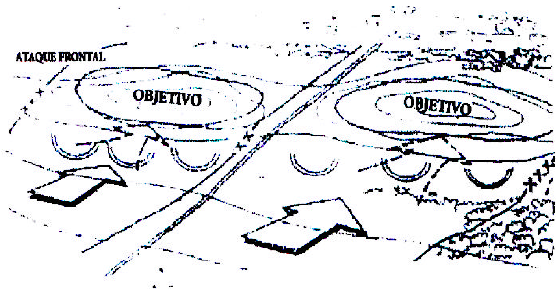
\includegraphics[scale=0.6]{\ruta/i/2/1/ataque-frontal.png}
 \caption{Maniobra frontal}
 \label{2-1:fig:ataque-frontal}
\end{figure}

\subsubsection{Maniobra envolvente}
La maniobra envolvente tiene como propósito evitar el ataque frontal del enemigo y cortar por las rutas de escape del enemigo desde los flancos o retaguardia.
\begin{figure}[H]
 \centering
 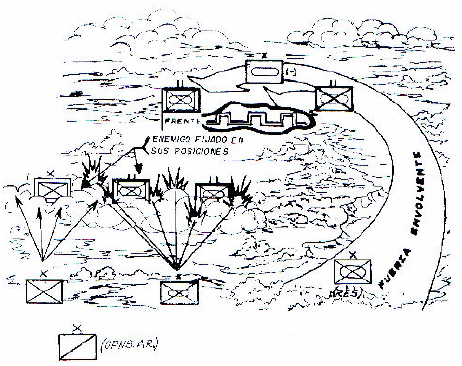
\includegraphics[scale=0.6]{\ruta/i/2/1/ataque-envolvente.png}
 \caption{Maniobra envolvente}
 \label{2-1:fig:ataque-envolvente}
\end{figure}


\subsubsection{Maniobra de ruptura}
El fin de la maniobra de ruptura es dividir la fuerza enemiga; busca llegar a la retaguardia enemiga a través de determinada zona del \gls{frente}.
\begin{figure}[H]
 \centering
 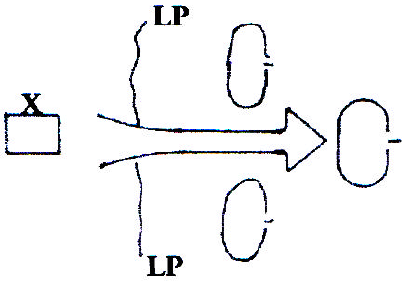
\includegraphics[scale=0.6]{\ruta/i/2/1/ataque-ruptura.png}
 \caption{Maniobra de ruptura}
 \label{2-1:fig:ataque-ruptura}
\end{figure}


%% >>>


\subsection{Operaciones defensivas}
Las operaciones defensivas se caracterizan por ser operaciones militares destinadas a resistir, rechazar o impedir el ataque de un enemigo.


\subsubsection{Defensa Móvil}
La defensa móvil se basa en el uso de fuerzas ofensivas de fácil desplazamiento para lograr la destrucción de fuerzas enemigas, es decir, su interés se centra en la eliminación del enemigo más que en el mantenimiento del terreno. Para ello, se utiliza el mínimo de unidades en el \gls{frente} de la unidades propias y se busca aprovechar el terreno para lograr cubrir el \gls{frente} enemigo con el resto de unidades.
\begin{figure}[H]
 \centering
 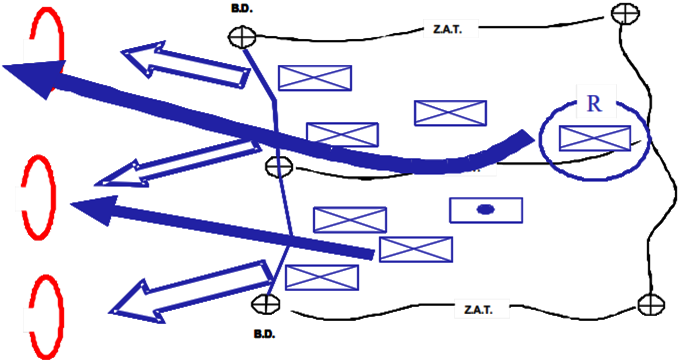
\includegraphics[scale=0.4]{\ruta/i/2/1/defensa-movil.png}
 \caption{Defensa móvil}
 \label{2-1:fig:defensa-movil}
\end{figure}

\subsubsection{Defensa de Área}
La defensa de área toma por objetivo mantener o controlar un terreno específico durante un determinado tiempo, en el cual las unidades y armamentos son importantes para detener o rechazar al atacante del área de avanzada\footnote{Porción del terreno por el cual se acercan los enemigos}. Para lograr la defensa de área, el estratega militar se prepara para aceptar el combate y evitar el avance enemigo, planificando el contra-ataque con el cual e rechaza o destruye a los enemigos.
\begin{figure}[H]
 \centering
 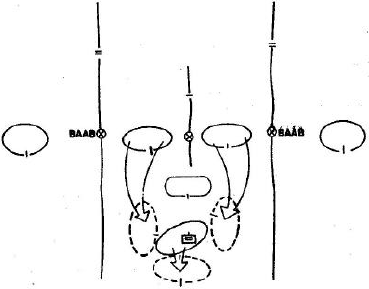
\includegraphics[scale=0.6]{\ruta/i/2/1/defensa-area.png}
 \caption{Defensa de zona}
 \label{2-1:fig:defensa-zona}
\end{figure}


%% >>>


\subsection{Operaciones retrógradas}
El propósito de las operaciones retrógradas es preservar las unidades y armamentos hasta obtener condiciones favorables para el ataque.

\subsubsection{Acción retardatriz}
La acción retardatriz se basa en mantener un ataque constante al enemigo, durante un tiempo determinado, pero sin la decisión de acabar con él.

\subsubsection{Repliegue}
El repliegue se aplica retirando parte o todas las unidades que están cerca al enemigo.

\subsubsection{Retirada}
La retirada se realiza para evitar el combate, bajo las condiciones existentes.

%%% Local Variables:
%%% mode: latex
%%% TeX-master: "../../tesis"
%%% End:
